\subsubsection{EndOfLine to PureCircuit Constant Parsimonious Reduction}

We will define the necessary prerequisites for the current section:

\begin{definition}[Poly-Function Bounded Parsimonious Reductions]
    Given two counting problems $A, B : \{0,1\}* \to \mathbb{N}$
    and a function $f : {0,1}^{*} \to \mathbb{N}$ such that $f \in n^{O(1)}$, we
    say that:
    $$
    A \subseteq^f B
    $$
    If for input $w \in \{0,1\}^*$, if $a$ represent the number of solutions
    for problem $A$ and $b$ the number of solutions for problem $B$, we have:
    $$
    a \leq b \leq f(|w|) \cdot a
    $$
\end{definition}

\begin{proposition}[EndOfLine to 3D-StrongSperner Parsimonious reduction]
    $$
    \scn{\#EndOfLine} \subseteq \scn{\#3D-StrongSperner}
    $$
\end{proposition}

The above has been shown by %% Insert citation
Our main contribution comes from the following theorem


\begin{theorem}[3D-StrongnSperner to PureCircuit]
    Given $f(\cdot) = 20$, we argue
    $$
    \scn{\#3D-StrongSperner} \subseteq^f \scn{\#PureCircuit}
    $$
    Where $\scn{3D-StrongSperner}$ is represented as a tuple $(\lambda, 0^n)$
    where $n$ corresponds to grid size of $2^n$.
\end{theorem}

To show the above holds true we will first show the construction and
prove its correctness.
To simplify the counting argument, we modify a solution of $\textsc{3D-StrongSperner}$
as such: Assuming $S \subseteq \{0,1\}^n$ is the set of all solutions, such that we define $S$ as such:

\begin{align*}
    S &\triangleq \Big\{(i,j,k) \in (\{0,1\}^{n})^3 \mid  \\
      &\{\lambda(i + x_1, j + x_2, k + x_3) \mid x \in \{0,1\}^3 \}\Big\} \text{ covers all labels}
\end{align*}

We will create $\Lambda: (\{0,1\}^{(n+1)})^3 \to \{-1, +1\}^3$ such that
 
$$
    \forall (i,j,k) \in (\{0,1\}^{(n+1)})^3: \Lambda(i,j,k) \triangleq 
\lambda\left( \left\lfloor  \frac{{i+1}}{2}  \right\rfloor, \left\lfloor  \frac{{j+1}}{2} \right\rfloor, \left\lfloor  \frac{{k+1}}{2} \right\rfloor \right)  \\
$$

Conversely we can say that we map from our original domain to our new domain as such

$$
\forall  x \in \{ 0,1 \}^{3n}, i \subseteq \{ 0,1,2 \}: \lambda(x_{-i}, x_{i}) \to \Lambda(2x_{i}, 2x_{-i} -1)
$$

The above transformation can be visualised using the following figure

\begin{figure}[h!]
    \centering
    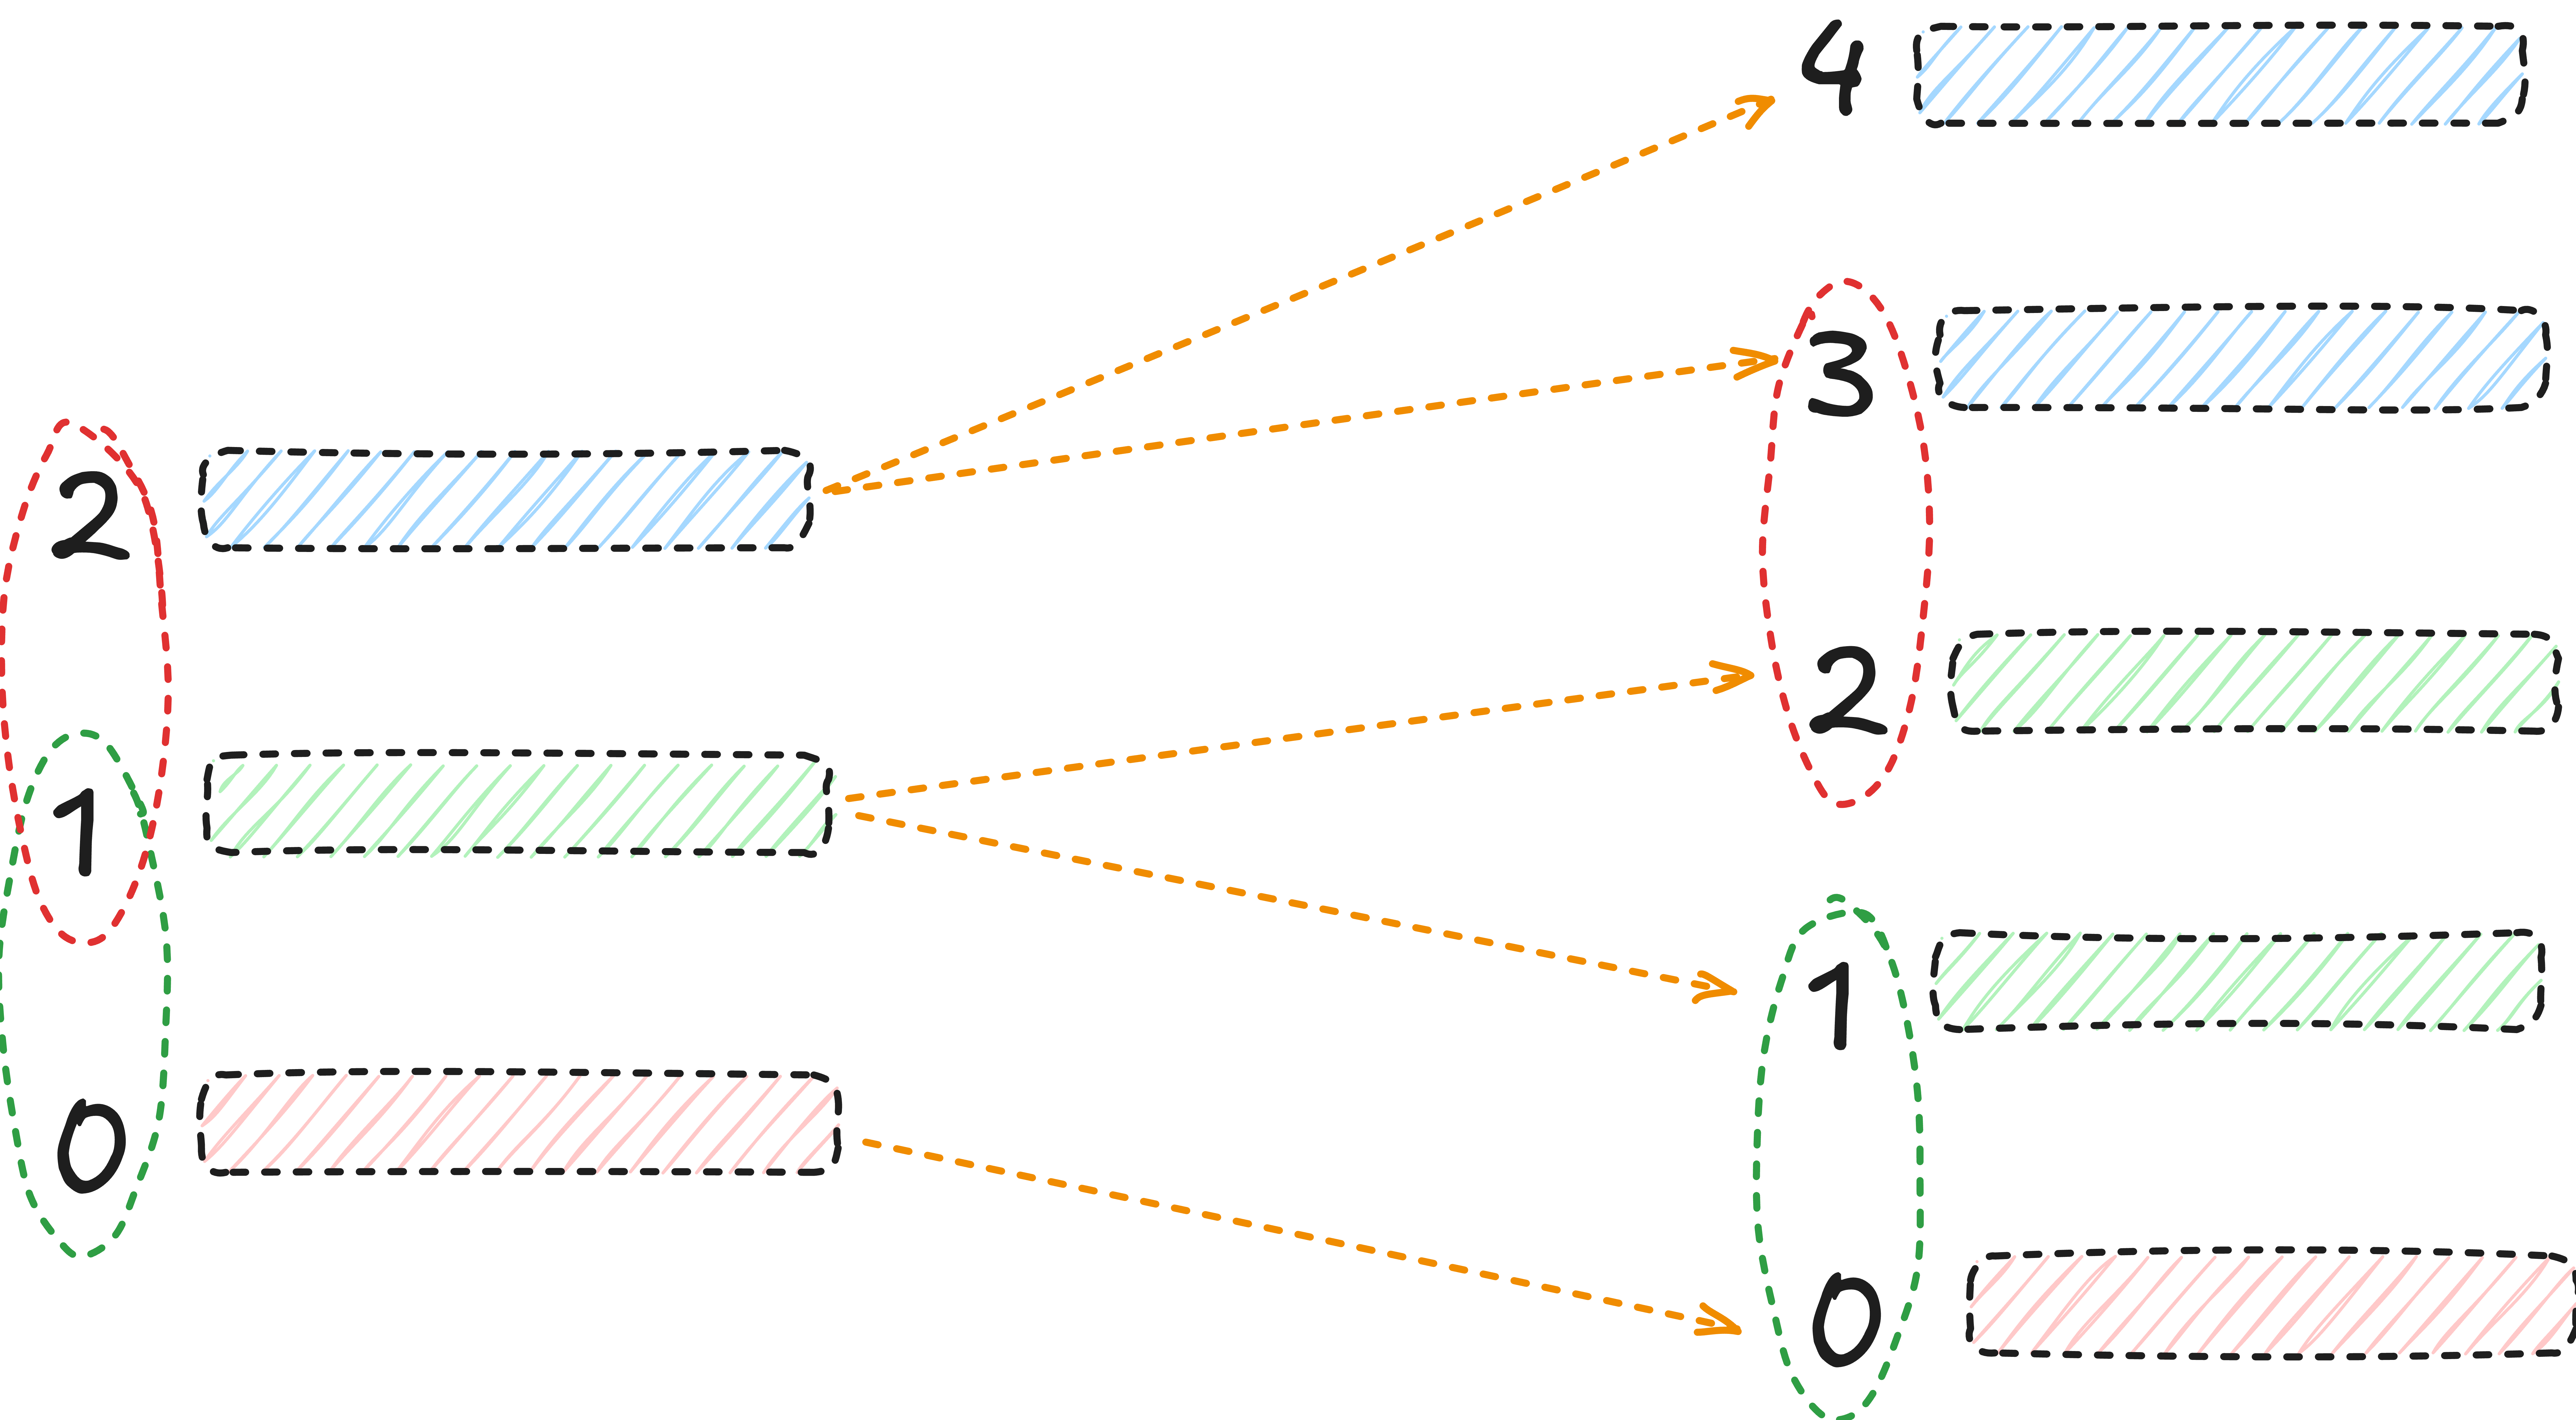
\includegraphics[width=0.5\textwidth]{assets/1751381227.png}
    \caption{The current figure allows depicts how solutions or pairs of solutions are mapped. For example for cube starting at 
        $i = 0$ and $i = 1$, we now just have to look at $i = 0$ and $i = 2$.}
    \label{fig:main-proof:set_mapping}
\end{figure}


\begin{claim}[Transformation claim]
    \label{clm:main-proof:trans-claim}
    We claim that $|S_{\text{even}}| = |S|$ where $S_{\text{even}}$  is defined as:
    $$
S_{\text{even}} \triangleq
   \Big\{(i0,j0,k0) \in (\{0,1\}^{(n+1)})^3 \mid  \\
   \{\Lambda(2i + x_1, 2j + x_2, 2k + x_3) \mid x \in \{0,1\}^3 \}\Big\} \text{ covers all labels}
    $$
\end{claim}

\begin{proof}
    We argue that we have a bijective transformation $S \leftrightarrow S_{\text{even}}$. To do that we will
    first show that every point in $x \in S$ is mapped to a single point in $x' \in S_{\text{even}}$.
    Assume $(i,j,k) = x$ for some $i,j,k \in \{0,1\}^{n}$. For a point to be in $S_{\text{even}}$
    has to be the case all 3 coordinates are even. From our transformation, there is only one mapping
    that achieves that, which is when $j = \{1,2,3\}$. We have to verify that this point corresponds to the
    same set of points or when $x' = (2i , 2j, 2k)$. We can observe its neighbourhood set:
    $$
    \Big\{\Lambda(2i + x_1, 2j + x_2, 2k + x_3) \mid x \in \{0,1\}^3 \Big\}
    $$
    We can observe that if $x_i = 1$ for any $i \in {1,2,3}$, that points
    corresponds to the same point as in $i + 1$. This implies that the set above
    corresponds to the neighbourhood:
    $$
    \Big\{\lambda(i + x_i, j + x_j, k + x_k) \mid x \in \{0,1\}^3 \Big\}
    $$
    And therefore the points match. We can conversely use the same argument to show the opposite
    direction and therefore we can conclude that $|S| = |S_{\text{even}}|$
\end{proof}
For simplicity's sake I will rename $n + 1$ as $n$ to keep the notation consistent.
Given the above we provide a main sketch of our tranformation as such:
\begin{enumerate}
    \item \textbf{Input bits}: We initialize input nodes $s_1, s_2, s_3$
    \item \textbf{Bit generator}: We apply the \textit{Bit Generator gadget} $\hat{P}$ for each $s_i$,
        to create numbers $u^1, u^2, u^3 \in \{0,1\}^{k}$
    \item \textbf{Circuit application}: We apply circuit modified circuit $\bar{\Lambda}$ to $u^1, u^2, u^3$ to create output values $o_1, o_2, o_3$
    \item \textbf{Validation}: Copy the results back to $s_1, s_2, s_3$
\end{enumerate}

The goal of the above transformation is to show that if $o_1 = o_2 =o_3 = \bot$, then we have a solution
to the original instance. The current construction allows us to match a single box of the original problem to
up to $20$ solutions of the PureCircuit one. We can visualise it as such:


\begin{figure}[h!]
    \centering
    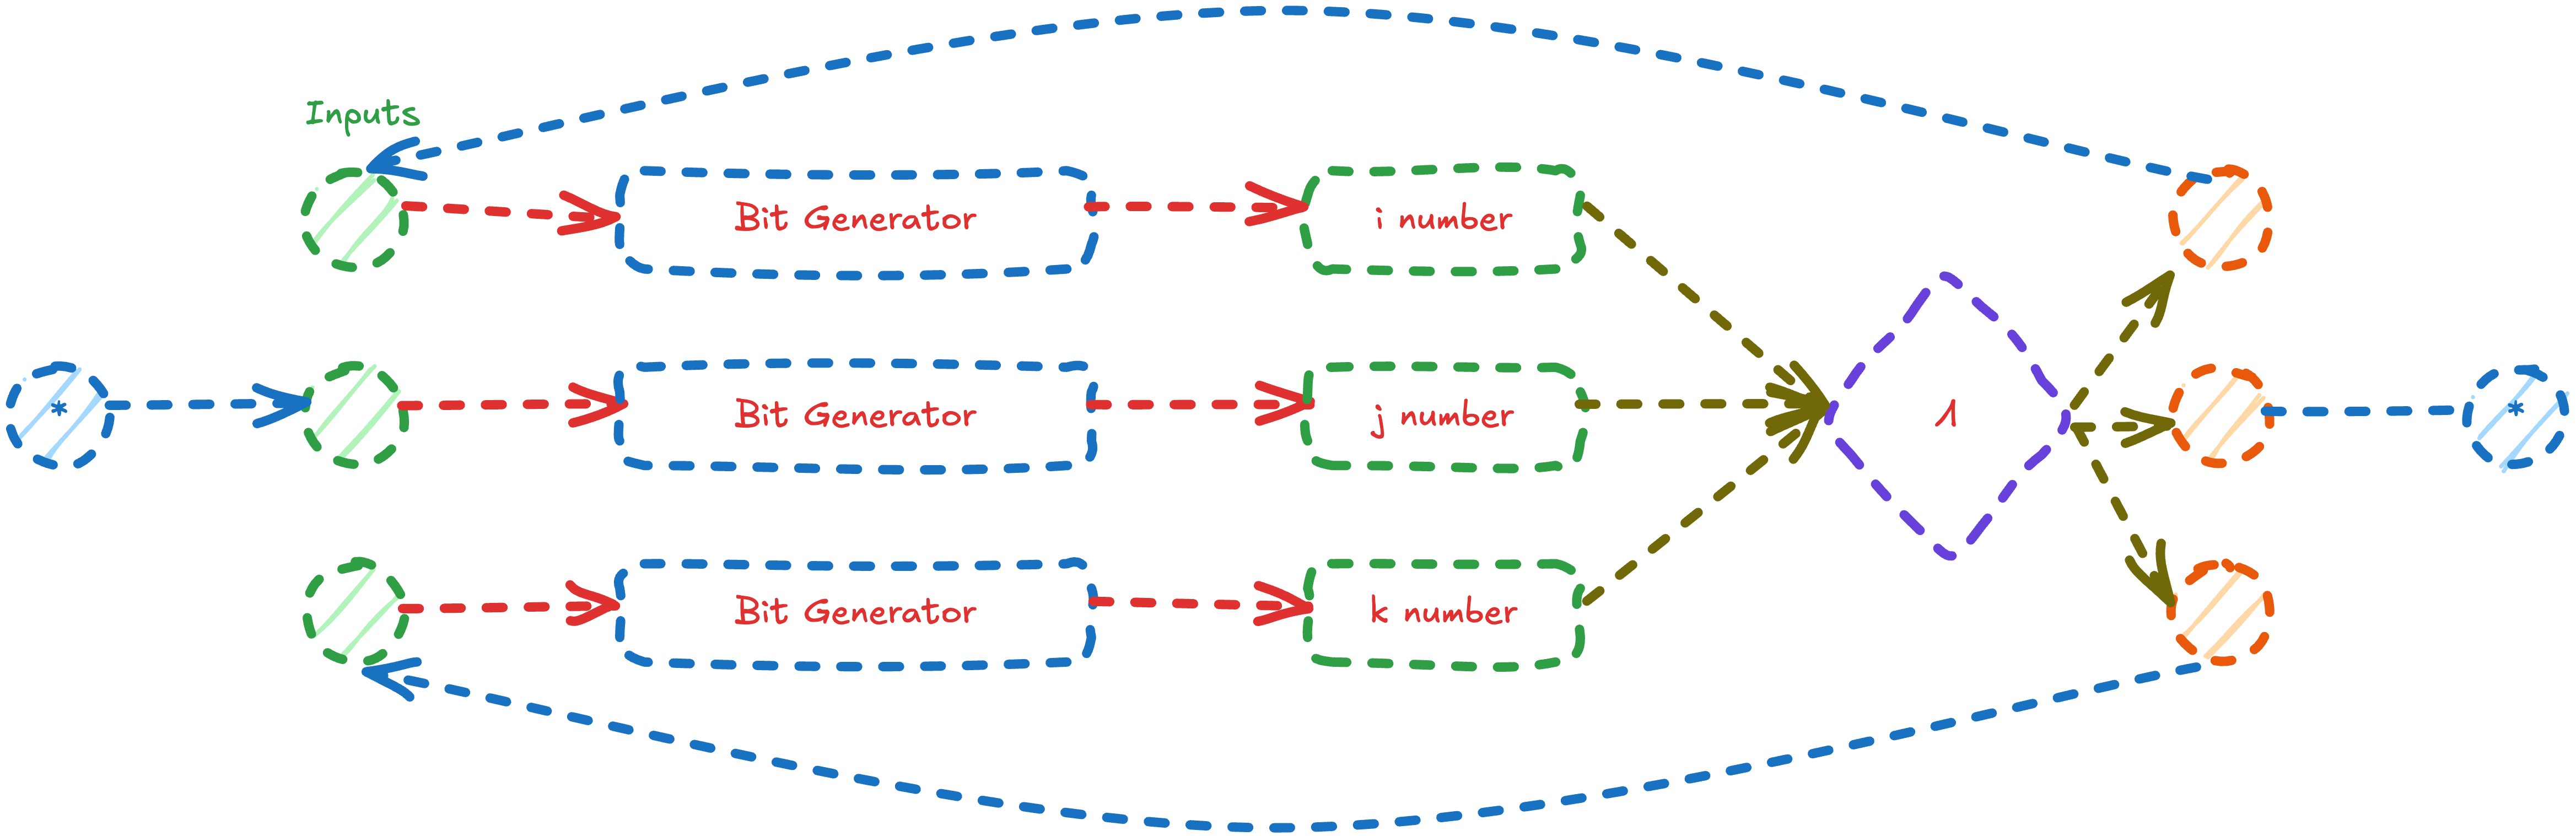
\includegraphics[width=0.75\textwidth]{assets/reduction_sketch.png}
    \caption{Testing}
    \label{fig:main-proof:visualisation}
\end{figure}


Before we look at the construction, we will refer to the standard set of gates $\{*, + , \neg\}$. These can
be trivially build using $\text{NOR}$ gates. Lastly we only accept the following as valid outputs of
the \textit{Purify} gate: $(0, \bot), (1, \bot), (\bot,1), (0,1)$. It is easy to see that for these set
of outputs, \textit{PureCircuit} remains \textbf{PPAD}-complete, by using the continuity argument.



\paragraph{Bit generator}

In order to generate our number we use the construction shown in the label \ref{fig:main-proof:purification},

\begin{figure}[h!]
    \centering
    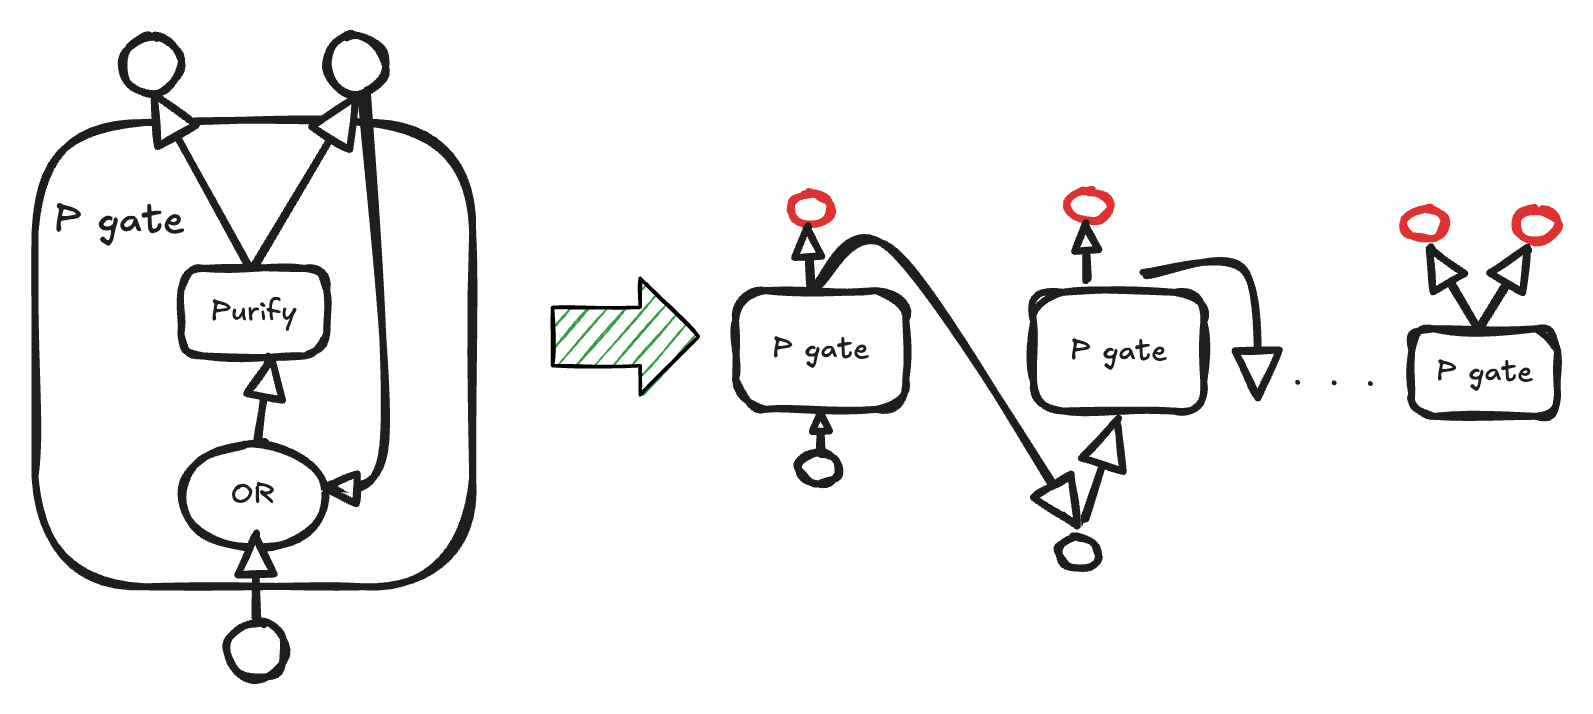
\includegraphics[width=0.5\textwidth, clip]{assets/purification_generator.png}
    \caption{Our bit generator bit is stacked version of a lot of $\hat{P}$ circuits. Be stacking them as shown in the figure and choosing the red nodes,
    we get our binary number.}
    \label{fig:main-proof:purification}
\end{figure}
\FloatBarrier

Given that construction we make the following lemma

\begin{lemma}[Bit Generator Lemma]
    \label{lem:bit-gen}
    The following hold true in our construction:
    \begin{enumerate}
        \item if $s_i = b \implies u^i = b^n$, given $b \in \mathbb{B}$
        \item if $s_i = \bot \implies \forall j \in [n-1]: u^i_j \in \mathbb{B}$ and $u^i_{n} \in \{1, \bot\}$
    \end{enumerate}
    We essentially ensure that if there exists a $\bot$ in our numbe, it should only be found in the last digit
\end{lemma}

\begin{proof}
    The first part follows trivially from the defintion of the \scn{Purify} gate, therefore if our input is a pure bit,
    we are copying it to all the inputs. To prove the second part of lemma, we use assume contradiction.
    Assume $\exists j \in [n-1]$. That would imply that one of the purify gates had an output of $(\bot, 1)$.
    But due to our $\textsc{OR}$ gate, that would force the input to be $1$ which would imply that the output is $1,1$.
    This implies that the only bit that can be $\bot$ is the last bit.
\end{proof}




\paragraph{Circuit Application}

In the current phase, we will modify the circuit $\Lambda$ to be hazard-free using the construction
from the \textit{Corollary 10} of \cite{ikenmeyerComplexityHazardfreeCircuits2019}.
They showed that we can ensure a k-bit hazard-free circuit with the following properties:

\begin{align*}
\text{size}(C)  & =  \left( \frac{ne}{k}  \right)^{2k} (|C| + 6) + O (n^{2.71k}) \\
\text{depth}(C)  & =  D + 8k + O(k \log n)
\end{align*}

Using the bit generator lemma \ref{lem:bit-gen}, we can observe that we can have at most 3 $\bot$ values 
in our input. This implies that we can create a circuit of polynomial size such that it is hazard-free.
Using that property we create the lemma below:

\begin{lemma}[Circuit Application Lemma]
    \label{lem:circuit}
    If $o_1 = o_2 = o_3 = \bot$ implies that we covered all the labels and found a solution
    in $(i0,j0,k0) \in P_{\text{even}}$
\end{lemma}


\begin{proof}
    First part is to understand what our $u^{(1)}, u^{(2)}, u^{(3)}$
    represent. To do that, we use the following visualisation on the figure \ref{fig:main-proof:cube-vis}
    \begin{figure}[h!]
        \centering
        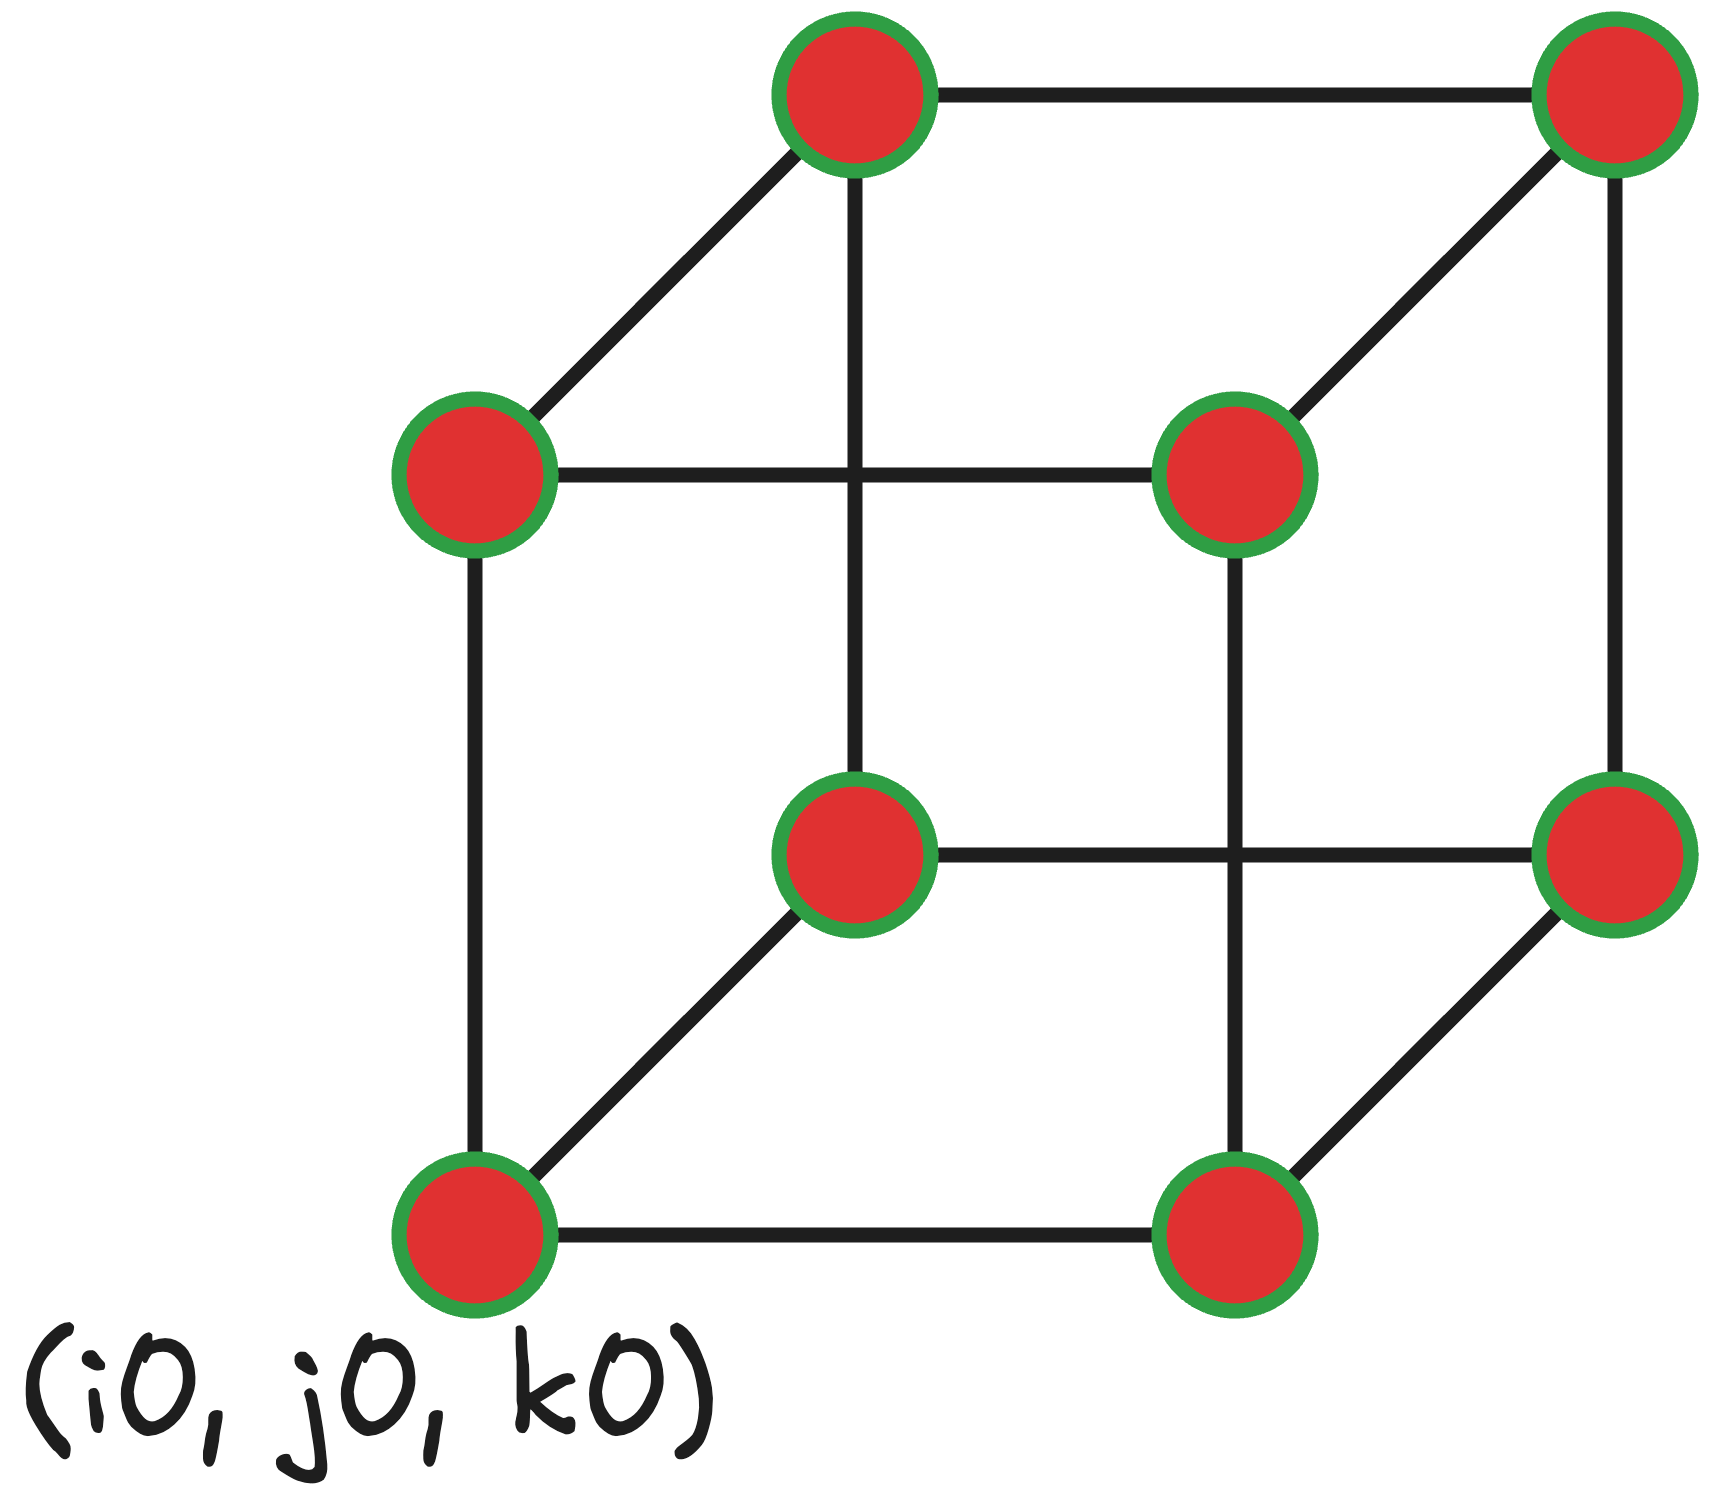
\includegraphics[width=0.2\textwidth]{assets/3d-cube.png}
        \caption{Representation of our solutions}\label{fig:main-proof:cube-vis}
    \end{figure}
    The first $n-1$ bits denote the $i,j,k$ indexes of our original solution.
    The cube essentially represents all possible realisations of $i\bot, j\bot, k\bot$.
    We know that the neighbouring corners correspond to vertices in our original instance.
    When all LSBs are $\bot$, we can observe that we are calculating our $\Lambda(\cdot)$
    for all corners of the cube simultaneously. If $(i0, j0, k0)$ is a solution
    that implies:
    $$
    \forall i \in \{1,2,3\}, b \in \{-1, 1\} \exists c \in \textsc{Res}(i\bot, j\bot, k\bot): [\bar{\Lambda}(c)]_i = b
    $$
    That implies if $\bar{\Lambda}$ outputs $\bot$ in some dimensions, then it found two points with different labels. We can therefore
    argue that if the output it $\bot^3$, then we covered all the labels.
\end{proof}


The above section conclude our construction. We will now demonstrate the correctness argument:

\begin{lemma}[Correctness lemma]
    We argue that every correct assingment of the above circuit, corresponds to a point in $P_{\text{even}}$
\end{lemma}
From the transformation claim \ref{clm:main-proof:trans-claim}, we know that if our circuit
can find all corresponding points in $P_{\text{even}}$, we can find the all the solutions of the original circuit.

\begin{proof}
    To prove our lemma, it suffices to show that $o_1 = o_2 = o_3 = \bot$. Let's assume by contradiction that
    $\exists i \in \{1,2,3\}$ such that label $i$ is not covered, meaning $o_i \neq \bot$.
    WLOG assume that $o_i = 0$. Our verification stage, will copy $0$ onto $s_i$. By our
    bit generator lemma \ref{lem:bit-gen}, we have that $u^{(i)} = 1^n$. From the boundary
    conditions of our circuits, and the k-bit hazard-freeness construction by
    \ref{lem:circuit}, we know that $\Lambda(*, 0^n, *) = \{*, 1,  *\}$. But that implies
    $o_i = 1$ which leads to a contradiction. We can make a similar argument to when $o_i = 1$.
\end{proof}

\paragraph*{Counting Argument}

To find how many solutions correspond to a single solution of the original instance,
we can make the following observation: Looking at our cube \ref{fig:main-proof:cube-vis},
if a side of the cube contains all labels, or if an edge contains all labels, we are counting
those as additional solutions. We can find an upper bound by making the following observation:

$$
\underbrace{\binom{3}{1} \cdot 2}_{\substack{\text{One of the sides is odd} \\ \text{and covers all labels}}}
+ \underbrace{\binom{3}{2} \cdot 2^2}_{\substack{\text{One of the edges is odd} \\ \text{and covers all labels}}}
+ \underbrace{1}_{\text{All LSBs are } \bot} = 20
$$

Therefore, we can bound the number of solutions of \textsc{3D-StrongSperner} by a factor of 20.
Core breakthorugh came from the utilisation of the hazard-freeness from \cite{ikenmeyerComplexityHazardfreeCircuits2019},
as well as studying some problems in EOPL and UEOPL or more specifically the
One-Permutation Discrete map. Athough in the end we were not able to extract any significantlly
useful results out of it, its key observations were enough.


\paragraph*{Useful Corollaries}
We can easily observe that our reduction above can work with any dimensionality.
In fact for any $\forall n in \mathbb{N}_{\geq 2}$, Chen et al. showed that
$\textsc{nD-StrongSperner}$ is still \textit{PPAD-Hard}. Additionally based on our proof, 
we can make the following corollary:

\begin{corollary}
Given $\scn{nD-StrongSperner}$, we define $f$ as:
$$
f(\cdot) = \sum_{i = 1}^{n - 1}2^k
$$
Such that we have the following relationo
$$
\scn{\#nD-StrongSperner} \subseteq^f \scn{\#PureCircuit}
$$
\end{corollary}

In addition we know that (INSERT CITATION), found a parsimonious
reduction from the $\textit{EndOfLine}$  to $\scn{3D-StrongSperner}$,
using a slighgly different colour scheme. One can use the same construction
that was done on the $\scn{2D-StrongSperner}$ to show \textsc{PPAD-Hardness}
by Chen et al. by using a different but very similar variant to the $\textsc{EndOfLine}$.
Lastly we conjecture that we can use the snake embedding technique by Chen Et Al. to bound
all the $\scn{ND-StrongSperner}$ to the same bounds as the $\scn{2D-StrongSperner}$.
More formally we conjecture the following to be true

\begin{conjecture}
\begin{gather*}
    f(\cdot) = \binom{2}{1} * 2 + 1 \\
    \forall n \in \mathbb{N}_{\geq 2} : \scn{\#nD-StrongSperner} \subseteq^f \scn{\#PureCircuit}  
\end{gather*}
\end{conjecture}

\subsubsection{Hazard-Free Logic Findings}

Whilst trying to tackle the main objectives of the dissertation, we stumbled upon
several interest relations across Hazard. We will use the notion of
promise problems to show the following relation. First we will
define a variant of UnSAT hazard as explained in \cite{ikenmeyerComplexityHazardfreeCircuits2019}.

\begin{definition}
    Given a circuit $C$ that computes $f : \mathbb{B}^n \to \mathbb{B}$ such that
    $\forall x \in \mathbb{B}^n : f(x) = 0$, find $\bar{x} \in \mathbb{T}^n$ such that
    $C(\bar{x}) = \bot$. We assume that $\forall x \in \mathbb{B}^n: C(x) = 0$.
\end{definition}

Given the idea above we propose the following:

\begin{proposition}
    $$
        \scn{\#PromiseUnsatHazard} \subseteq  \scn{\#PureCircuit} -1
    $$
\end{proposition}

For the purposes of the current reduction, we will use the same \textsc{Purify} values
$(0,1), (0,\bot), (1,\bot), (\bot, 1)$

\paragraph{Construction}
We start with a single node $s$. We create $n$ copies of \textsc{Purify}, where all 
use $s$ as the input. From each purify gate we use the left output and
create a vector $\hat{x} \in \mathbb{T}^n$ and pass them
onto $C$ which will output onto a node $o$. We copy the output onto $s$.
The above description can be summarised in the following figure \ref{fig:unsat-proof}.

\begin{figure}[h!]
    \centering
        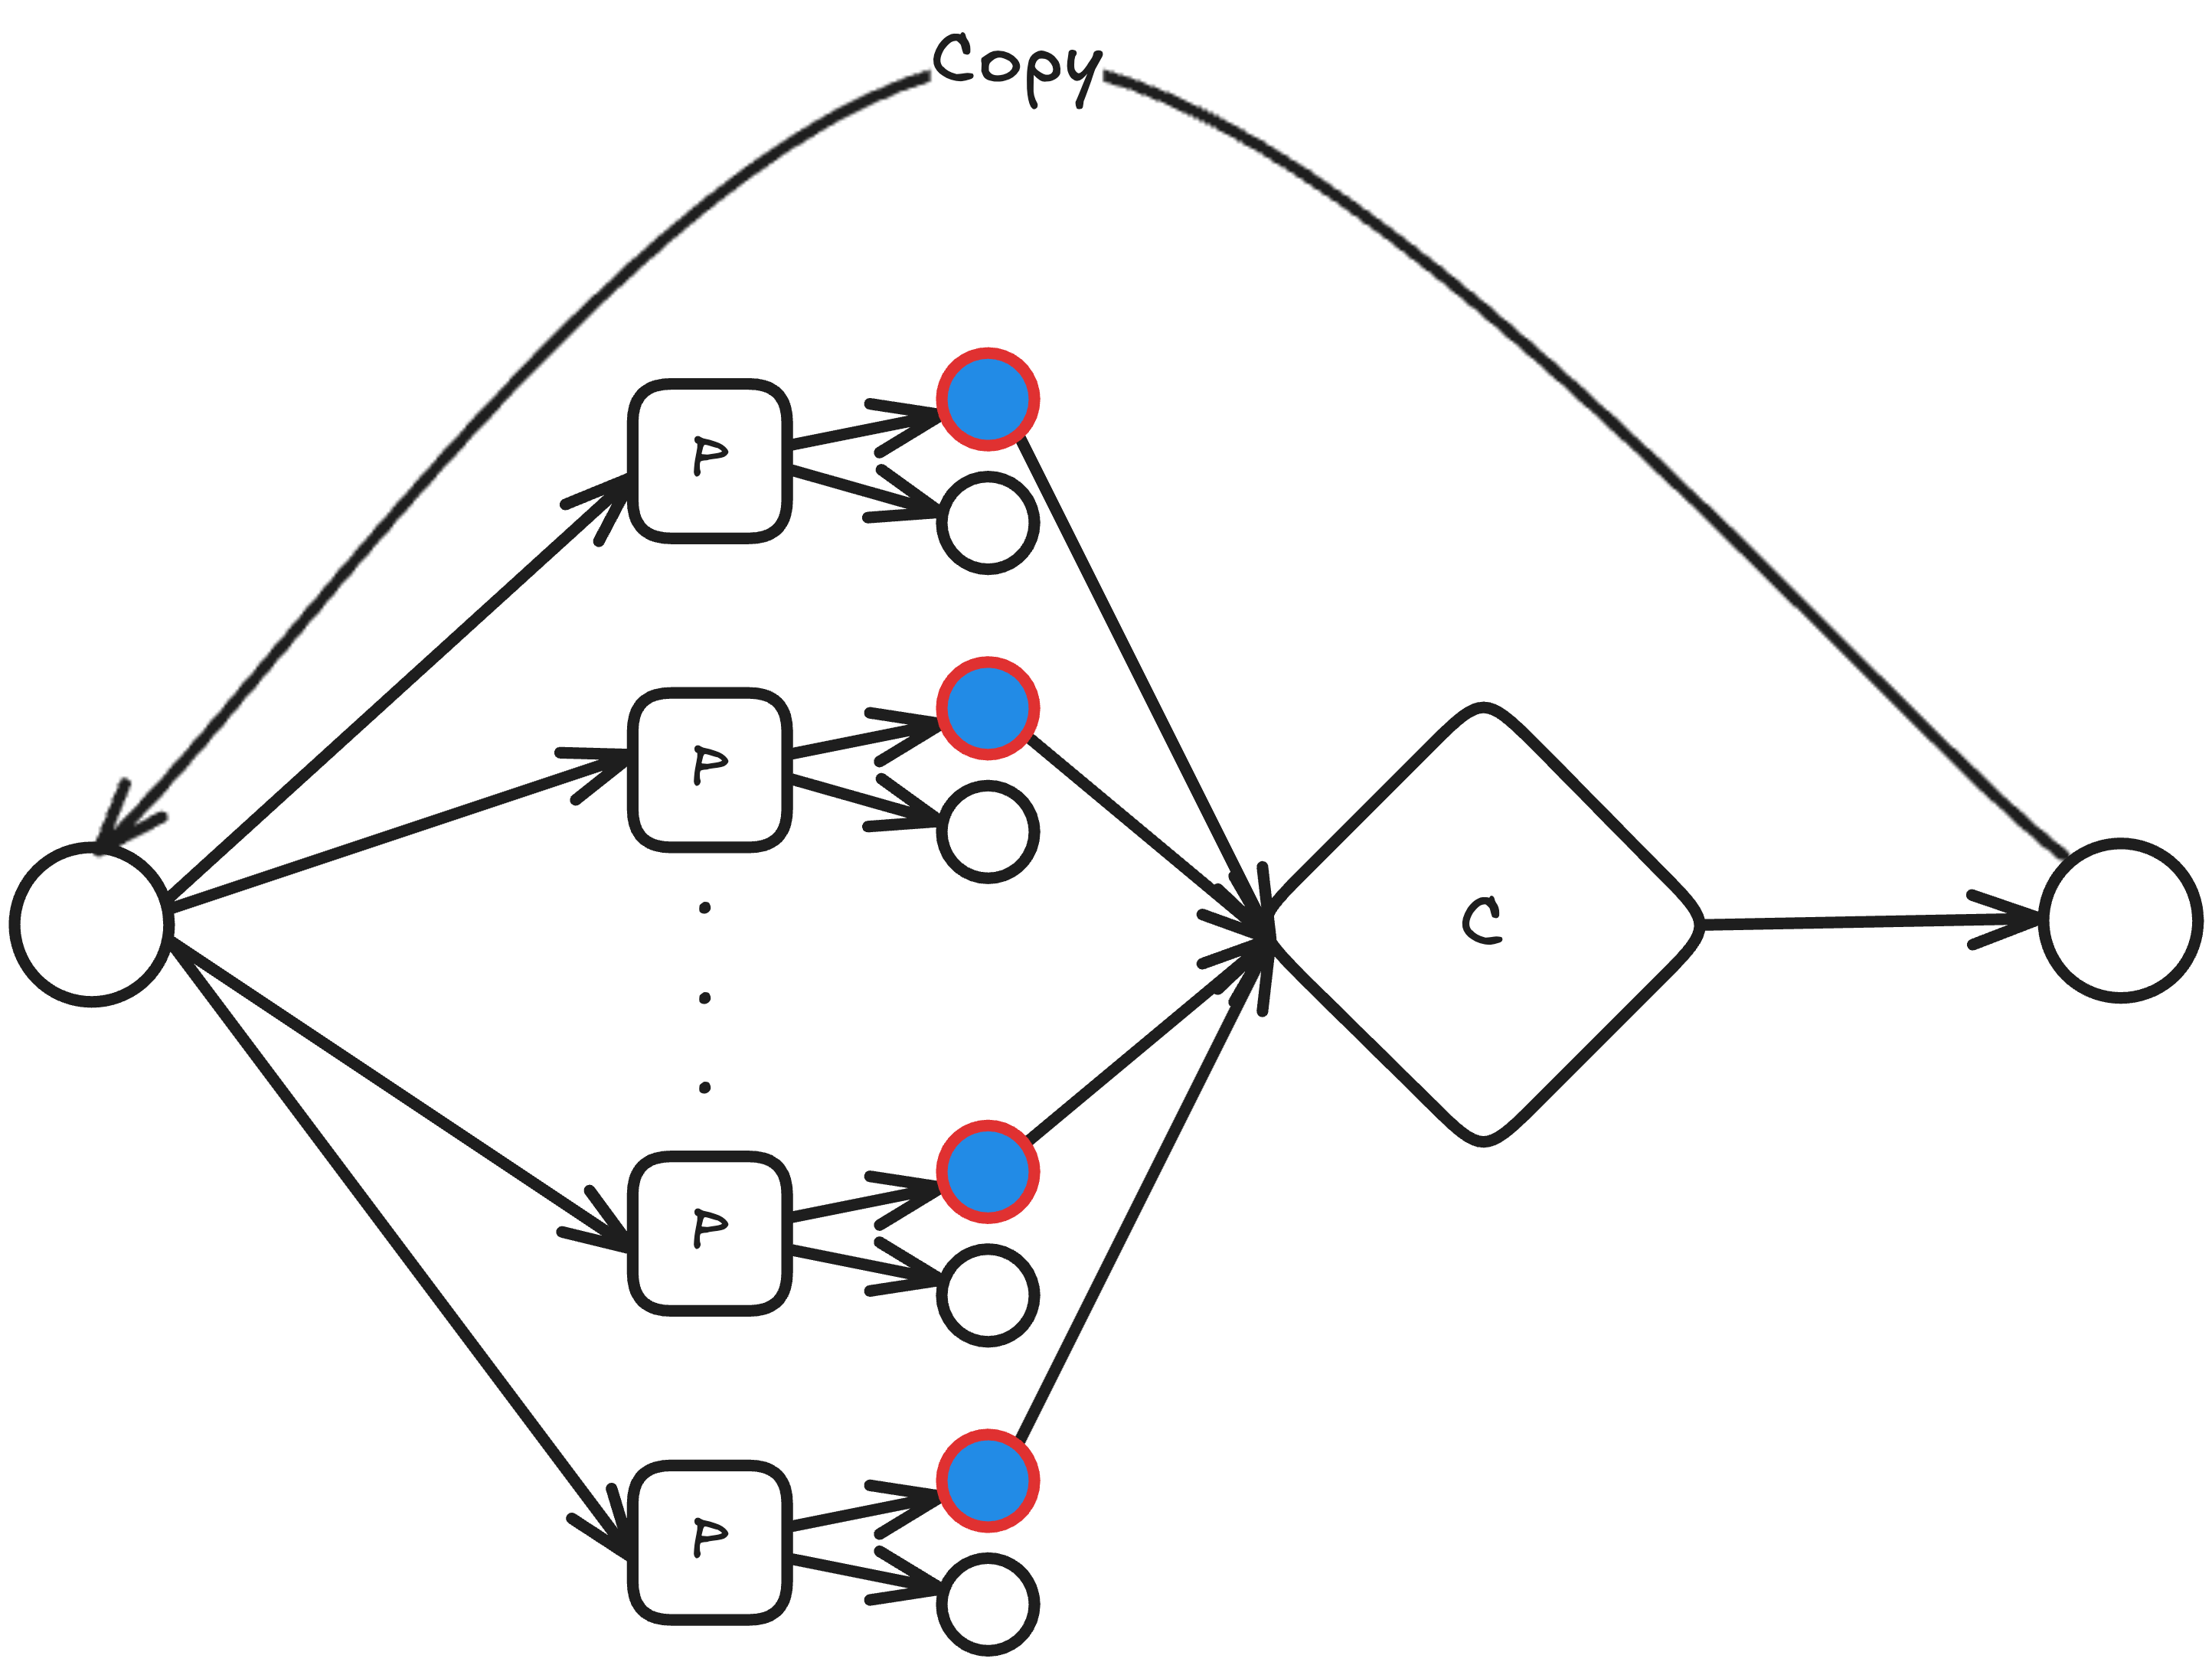
\includegraphics[width=0.5\textwidth]{assets/circuit-unsat.png}
    \caption{Pure Circuit construction}
    \label{fig:unsat-proof}
\end{figure}

\begin{proof}
To prove our counting argument, we can make the following observation:
If $o = 0$, we are computing $C(0^n) = 0$, which is the one guaranteed solution.
We know that $o \neq 1$, therefore the only other possible solutions are $\bar{x} \in \mathbb{T}^n: C(\bar{x}) = \bot$.
We also know from our construction of our \textsc{Purify} gate values, that our highlighted nodes
    can take values $\{0,1,\bot\}$. Therefore, given that $\hat{x} \in \mathbb{T}^n$,
our construction can find all possible solutions.
\end{proof}


\subsubsection{Hazard Circuits and Tarski}
The following finding was derived when looking into alternative fixed point problems.
In the following proposition we found a pretty interesting connection between
\textit{natural} functions and \textsc{Tarski}. More specifically, 
\textsc{Tarski} is a complexity problem in $\textsc{CLS}$. First
it is essential to define monotone functions:

\begin{definition}[Monotone functions]
    Given two posets $(L_1, \preceq_{L_1})$ and $(L_2, \preceq_{L_2})$, a function
    $f: L_1 \to L_2$ is \textbf{monotone} if and only if:
    $$
    \forall x,y \in L_1: x \preceq_{L_1} y \implies f(x) \preceq_{L_2} f(y)
    $$
\end{definition}
    



\begin{definition}[$\scn{Tarski}$ problem definition]
    Given a lattice $(L, \wedge, \vee)$, and a \textit{monotone} function $f : L \to L$,
    we define solutions to the problem as:
    \begin{enumerate}
        \item Find $x \in L: f(x) = x$
        \item Find $x,y \in L$ such that $x \preceq y$ and $f(x) \not\preceq f(y)$
    \end{enumerate}
\end{definition}


We can use the information ordering to impose a partial order on $(\mathbb{T}, \preceq)$ as such:
$$
\forall x,y \in \mathbb{T}^n : x \preceq y \implies \forall j \in [n]: x_j \in \mathbb{B} \implies x_j = y_j
$$

Therefore we create the following subclass of \textsc{Tarski}


\begin{definition}[$\scn{KleeneTarski}$ problem definition]
    Given $F: \mathbb{T}^n \to \mathbb{T}^n$, where $F$ is a \textit{natural} function,
    we want to find the set of points $\textbf{Fix}^\star$ such that
    $$
        \forall x \in \textbf{Fix}^\star: F(x)  = x
    $$
    We assume $F$ will be represented as a circuit, that uses
    $\{*, +, \neg, \mathbb{0}, \mathbb{1}\}$.
\end{definition}


\begin{proposition}[Parsimonious Reduction between $\scn{KleeneTarski}$ and $\scn{PureCircuit}$]
    $$
    \scn{\#KleeneTarski-1} \subseteq \scn{\#PureCircuit} -1
    $$
\end{proposition}

The above reduction can be done trivially using the following three steps:
\begin{enumerate}
    \item Initiate a vector of nodes $s$
    \item Pass the inputs into a circuit $C$ that computes the input into an output vector $o$
    \item Copy the results back into $s$
\end{enumerate}

We can observe that for any valid assignment, $\mathbf{x}[s]= \mathbf{x}[o]$.
Therefore, our construction can find all fix points for Kleene Circuits.

\subsubsection{Reductions to the EndOfLine}

One can also attempt to make some reductions to the \textsc{EndOfLine}. It has to be noted,
that we assume that there are no parsimonious reductions to the \textsc{EndOfLine},
but we were able to construct some variants that allows to make there reductions.
They key insights for this comes from the \textsc{PPAD}-inclusion proof
by Deligkas et al. \cite{deligkasPureCircuitTightInapproximability2024}, where they
showed that we can reduce PureCircuit, to \textit{Brouwer} problem by constructing
a continuous function $F: [0,1]^n \to [0,1]^n$ as such: For each $v \in V$, we create
continuous functions $f_i(\cdot): [0,1]^n \to [0,1]$ where we take thne input of vector
of all the nodes and output the value of the current node
\begin{enumerate}
    \item If $v \in V$ is the output of a $\textsc{NOR}$ gate with inputs $x_1, x_2$, then we have:
        $$
        f_v(\mathbf{x}) := (1 - \mathbf{x}_{x_1}) \cdot (1 - \mathbf{x}_{x_2})
        $$
    \item If $y_1, y_2$ are the outputs of a  $\textsc{Purify}$ gate with $z$ as input, then we have:
        \begin{align*}
            f_{y_1}(\mathbf{x}) &:= \max\{2 \cdot \mathbf{x}_{z} - 1, 0\}\\
            f_{y_2}(\mathbf{x}) &:= \min\{2 \cdot \mathbf{x}_{z}, 1\}
        \end{align*}
\end{enumerate}
If $F(x) = x$, then we also found a solution for \textsc{PureCircuit} by:
$$
\forall v \in V: \mathbf{x}[v] = \begin{cases}
    0 & \mathbf{x}[v] = 0 \\
    \bot & 0 < \mathbf{x}[v] < 1 \\
    1 & \mathbf{x}[v] = 1 \\
\end{cases}
$$
Given that as an assumption we can restrict our \textit{Purify} gate
to outputs $(0,\bot), (0,1), (\bot, 1)$. Using that we can define two types of variants
of \textsc{PureCircuit} that are parsimoniously reducible to \textsc{SourceOrPresink}.
We first define \textsc{SourceOrPresink} as:

\begin{definition}[$\scn{SourceOrPresink}$ definition]
    A $\scn{SourceOrPresink}$ is defined by the same construction as the $\scn{EndOfLine}$ 
    but the solutions are sources and predecessors of sinks. If a node is both a source
    and a presink, then we count it once.
\end{definition}

We will annotate our \textit{Purify} gates with an additional bit $b \in \mathbb{B}$ such that
$$
\forall x \in \mathbb{T}, y_1, y_2 \in \mathbb{T}: \textsc{Purify}^b(x) = (y_1,y_2) \implies \textsc{Purify}^{\neg {b}}(x) = (y_2, y_1)
$$
We can create two types of problems based on the annotation:
\begin{enumerate}
    \item Acyclic \textsc{PureCircuit}: Our instance is acyclic
    \item Permutation-free \textsc{PureCircuit}: The outputs of a pure circuit, are connected to a circuit such that any permutation of the inputs
        retains the result. More formally:
        $$
        \forall x \in \mathbb{T}^n, \sigma \in \mathcal{A}: C(\sigma(x)) = C(x)
        $$
        Where $\mathcal{A}$ is the set of automorphisms of $[n] \to [n]$.
        The above description can be depicted in the following figure:
        (ADD FIGURE)
\end{enumerate}

We can show that above variants we can create the following proposition (ref).
To prove the reduction we can need to argue that we can go from one solution to another.
The core idea of these problems is:  if we find a solution given in 
a set of configurations $\gamma \in \{0,1\}^p$ where $p$ are the number of purify gates,
we can match it with an additional solution where our set of configurations is $\neg \gamma$.
This can be visualised as such: If the flip does not affect the inputs then we
can create the following graph:

\begin{figure}[h!]
\centering


\tikzset{every picture/.style={line width=0.75pt}} %set default line width to 0.75pt        

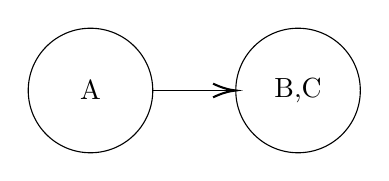
\begin{tikzpicture}[x=0.75pt,y=0.75pt,yscale=-1,xscale=1]
%uncomment if require: \path (0,260); %set diagram left start at 0, and has height of 260

%Shape: Circle [id:dp7760056968770814] 
\draw   (90,140) .. controls (90,123.43) and (103.43,110) .. (120,110) .. controls (136.57,110) and (150,123.43) .. (150,140) .. controls (150,156.57) and (136.57,170) .. (120,170) .. controls (103.43,170) and (90,156.57) .. (90,140) -- cycle ;

%Shape: Circle [id:dp22383258291194785] 
\draw   (190,140) .. controls (190,123.43) and (203.43,110) .. (220,110) .. controls (236.57,110) and (250,123.43) .. (250,140) .. controls (250,156.57) and (236.57,170) .. (220,170) .. controls (203.43,170) and (190,156.57) .. (190,140) -- cycle ;

%Straight Lines [id:da1444295916995948] 
\draw    (150,140) -- (188,140) ;
\draw [shift={(190,140)}, rotate = 180] [color={rgb, 255:red, 0; green, 0; blue, 0 }  ][line width=0.75]    (10.93,-3.29) .. controls (6.95,-1.4) and (3.31,-0.3) .. (0,0) .. controls (3.31,0.3) and (6.95,1.4) .. (10.93,3.29)   ;

% Text Node
\draw (120,140) node   [align=left] {A};
% Text Node
\draw (220,140) node   [align=left] {B,C};


\end{tikzpicture}
\caption{Equal solution conversion}
\label{fig:equal}
\end{figure}
Otherwise for two distinct solutions we can use the following
\begin{figure}[h!]
\centering
\tikzset{every picture/.style={line width=0.75pt}} %set default line width to 0.75pt
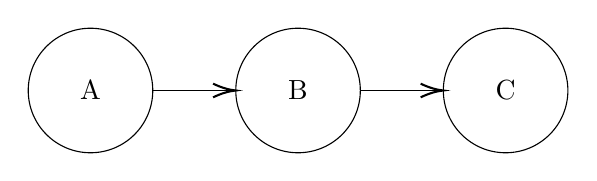
\begin{tikzpicture}[x=0.75pt,y=0.75pt,yscale=-1,xscale=1]
%uncomment if require: \path (0,260); %set diagram left start at 0, and has height of 260

%Shape: Circle [id:dp7760056968770814] 
\draw   (90,140) .. controls (90,123.43) and (103.43,110) .. (120,110) .. controls (136.57,110) and (150,123.43) .. (150,140) .. controls (150,156.57) and (136.57,170) .. (120,170) .. controls (103.43,170) and (90,156.57) .. (90,140) -- cycle ;

%Shape: Circle [id:dp22383258291194785] 
\draw   (190,140) .. controls (190,123.43) and (203.43,110) .. (220,110) .. controls (236.57,110) and (250,123.43) .. (250,140) .. controls (250,156.57) and (236.57,170) .. (220,170) .. controls (203.43,170) and (190,156.57) .. (190,140) -- cycle ;

%Shape: Circle [id:dp48038379742035975] 
\draw   (290,140) .. controls (290,123.43) and (303.43,110) .. (320,110) .. controls (336.57,110) and (350,123.43) .. (350,140) .. controls (350,156.57) and (336.57,170) .. (320,170) .. controls (303.43,170) and (290,156.57) .. (290,140) -- cycle ;

%Straight Lines [id:da1444295916995948] 
\draw    (150,140) -- (188,140) ;
\draw [shift={(190,140)}, rotate = 180] [color={rgb, 255:red, 0; green, 0; blue, 0 }  ][line width=0.75]    (10.93,-3.29) .. controls (6.95,-1.4) and (3.31,-0.3) .. (0,0) .. controls (3.31,0.3) and (6.95,1.4) .. (10.93,3.29)   ;
%Straight Lines [id:da6754989440526618] 
\draw    (250,140) -- (288,140) ;
\draw [shift={(290,140)}, rotate = 180] [color={rgb, 255:red, 0; green, 0; blue, 0 }  ][line width=0.75]    (10.93,-3.29) .. controls (6.95,-1.4) and (3.31,-0.3) .. (0,0) .. controls (3.31,0.3) and (6.95,1.4) .. (10.93,3.29)   ;

% Text Node
\draw (120,140) node   [align=left] {A};
% Text Node
\draw (220,140) node   [align=left] {B};
% Text Node
\draw (320,140) node   [align=left] {C};
\end{tikzpicture}
\caption{Not equal solution}
\label{fig:not-equal}
\end{figure}


\subsubsection{Next steps}

Our next steps will focus mainly on two directions. One is lowering the bound as we declare in our conjecture with the
usage of snake embeddings. We believe that each dimension can be parsimoniously reduced with another. This implies
that, if we can show that $\forall n \in \mathbb{N}_{\geq 3}: \textsc{\#nD-StrongSperner} \subseteq \textsc{\#2D-StrongSperner}$
we get to prove our conjecture.


With regards to, our second direction, we want to emphasize on the hardness of \textsc{PureCircuit}.
Or more specifically we will investigate as to if any of the following statements hold true.

\begin{gather*}
    \exists n, \alpha \in \mathbb{N}_{\geq 2}:
    \textsc{\#SourceOrExcess}(\alpha,1) - 1  \subseteq \textsc{\#nD-StrongSperner} -1 \\
    \exists n \in \mathbb{N}_{\geq 2}: \textsc{\#SourceOrExcess}(n,1) - 1 \subseteq \textsc{\#PureCircuit} -1 \\
\end{gather*}

We believe the above two should be our next steps in order to get close to the main question of our project.
Ideally generalising, the above reductions to the infinity hierarchy of
$\textsc{\#SourceOrExcess}(\cdot,1)$ would be ideal as it may lead to finding an overall upper bound
towards the entire $\textsc{\#PPAD} -1$ class.

